%//cSpell:disable
% LTeX: enabled=false
\documentclass[a4paper,ngerman, headheight=28pt,12pt]{scrartcl}


% PACKAGES
\usepackage[a4paper,left=3cm,right=4cm,top=2.5cm,bottom=2.5cm]{geometry}

\usepackage{fontspec}
\usepackage{babel}
\usepackage{csquotes}
\usepackage{svg}
\usepackage{relsize}
\usepackage{setspace}

\usepackage{lineno}

\usepackage{tabularray}
\usepackage{float}

% Appendix
\usepackage{appendix}

% Title Spacing

\RedeclareSectionCommand[
  %runin=false,
  afterindent=false,
  beforeskip=.5\baselineskip,
  afterskip=.25\baselineskip]{section}
\RedeclareSectionCommand[
  %runin=false,
  afterindent=false,
  beforeskip=.25\baselineskip,
  afterskip=.125\baselineskip]{subsection}
\RedeclareSectionCommand[
  %runin=false,
  afterindent=false,
  beforeskip=.175\baselineskip,
  afterskip=.0625\baselineskip]{subsubsection}


% Literaturverzeichnis
\usepackage[
backend=biber,
style=alphabetic,
sorting=nty,
maxbibnames=99
]{biblatex}

\addbibresource{refs_facharbeit.bib}

\DeclareLabelalphaTemplate{
  \labelelement{
    \field[final]{shorthand}
    \field{label}
    \field[strwidth=2,strside=left,ifnames=1]{labelname}
    \field[strwidth=1,strside=left]{labelname}
  }
  \labelelement{
    \field[strwidth=2,strside=right]{year}
  }
}
%//TODO Change font back to calibri
\IfFileExists{/etc/motd}{\setmainfont{calibri}[
  Path=./fonts/,
  Extension=.ttf,
  UprightFont=*-Regular,
  BoldFont=*-Bold,
  ItalicFont=*-Italic,
  BoldItalicFont=*-BoldItalic,
]}{\setmainfont{Calibri}}


\MakeOuterQuote{"}

\newcommand{\LongMinus}{–}

% LTeX: enabled=true
%//cSpell:enable
% Die nächsten vier Felder bitte anpassen:
\newcommand{\Titel}{Dezentralisierte asymmetrische \\ Verschlüsselung über Tor} % Titel für Facharbeit
\newcommand{\SubTitel}{Die Lösung für sicheres Messaging?}

\newcommand{\PageTitel}{Dezentralisierte asymmetrische Verschlüsselung \\ über Tor \LongMinus{} Die Lösung für sicheres Messaging?} % Seitentitel für Facharbeit
\newcommand{\Author}{Hendrik Lind}     % Ich
\newcommand{\Department}{Seminarfach Informatik}
\newcommand{\School}{Windthorst-Gymnasium Meppen}
\newcommand{\Country}{Deutschland}
\newcommand{\Abgabe}{20. November 2023}

\newcommand{\thesisDegree}{Facharbeit}
\newcommand{\faculty}{Seminarfach Informatik}
\newcommand{\thesisPlaceDate}{\today}

\newcommand{\vcite}[1]{\cite[vgl.][]{#1}}
\newcommand{\vebd}{[vgl. ebd.]}

% Tor Stuff
\newcommand{\entryn}{\textit{Entry Node\,}}
\newcommand{\relayn}{\textit{Relay Node\,}}
\newcommand{\relayns}{\textit{Relay Nodes\,}}
\newcommand{\exitn}{\textit{Exit Node\,}}
\newcommand{\exitns}{\textit{Exit Nodes\,}}
\newcommand{\nodes}{\textit{Nodes\,}}
\newcommand{\node}{\textit{Node\,}}
\newcommand{\onion}{\textit{Onion\,}}
\newcommand{\circuit}{\textit{Circuit\,}}
\newcommand{\circuits}{\textit{Circuits\,}}
\newcommand{\introp}{\textit{Introduction Point\,}}
\newcommand{\introps}{\textit{Introduction Points\,}}
\newcommand{\renp}{\textit{Rendezvous Point\,}}

% Implementation stuff
\newcommand{\identity}{\textit{Identity\,}}

%//cSpell:disable
% LTeX: enabled=false

% Kopf- und Fußzeilen
\usepackage{scrlayer-scrpage, lastpage}
\setkomafont{pageheadfoot}{\large\textrm}
\lohead{\PageTitel}
\rohead{\Author}
\cfoot*{\thepage{}/\pageref{LastPageDoc}}

% Position des Titels
\usepackage{titling}
\setlength{\droptitle}{-1.0cm}


% Für mathematische Befehle und Symbole
\usepackage{amsmath}
\usepackage{amssymb}
\usepackage{wrapfig}

% Für Bilder
\usepackage{graphicx}
\usepackage{graphbox}

% Für Algorithmen
\usepackage{algpseudocode}

% Für Quelltext
\usepackage{listings}
\usepackage{color}

% Für PDF
\usepackage{pdfpages}

\graphicspath{ {./img/} }


% 1.5 Line spacing
\setstretch{1.5}


% Umlaute erlauben
\lstset{literate=%
  {Ö}{{\"O}}1
  {Ä}{{\"A}}1
  {Ü}{{\"U}}1
  {ß}{{\ss}}1
  {ü}{{\"u}}1
  {ä}{{\"a}}1
  {ö}{{\"o}}1
}
%end


% Diese beiden Pakete müssen zuletzt geladen werden
\usepackage[hidelinks]{hyperref} % Anklickbare Links im Dokument
\usepackage{cleveref}

% Für Code
\usepackage[outputdir=build]{minted}


% Titlepage required things


% Necessary packages for the titlepage:
\usepackage{tikz}
\usetikzlibrary{calc}
%\usepackage{graphicx}
% \usepackage{newtxtext}
%\usepackage{float}
\usepackage{comment}
% This command changes the font style where SLU promotes Arial
%\newenvironment{myfont}{\fontfamily{phv}\selectfont}{\par}


% Add line breaks to urls
\apptocmd{\UrlBreaks}{\do\f\do\m}{}{}
\setcounter{biburllcpenalty}{9000}% Kleinbuchstaben
\setcounter{biburlucpenalty}{9000}% Großbuchstaben

% Optionally show or hide code

\newif\ifshow % toggle true or false based on if want to hide section
%\showtrue % show the sections
\showfalse % hide the sections

\usepackage{version}
\ifshow
  \includeversion{minted}
  \includeversion{wrap}
  \includeversion{equation}
\else
  \excludeversion{minted}
  \excludeversion{wrap}
  \excludeversion{equation}
\fi


% Facharbeit

\begin{document}
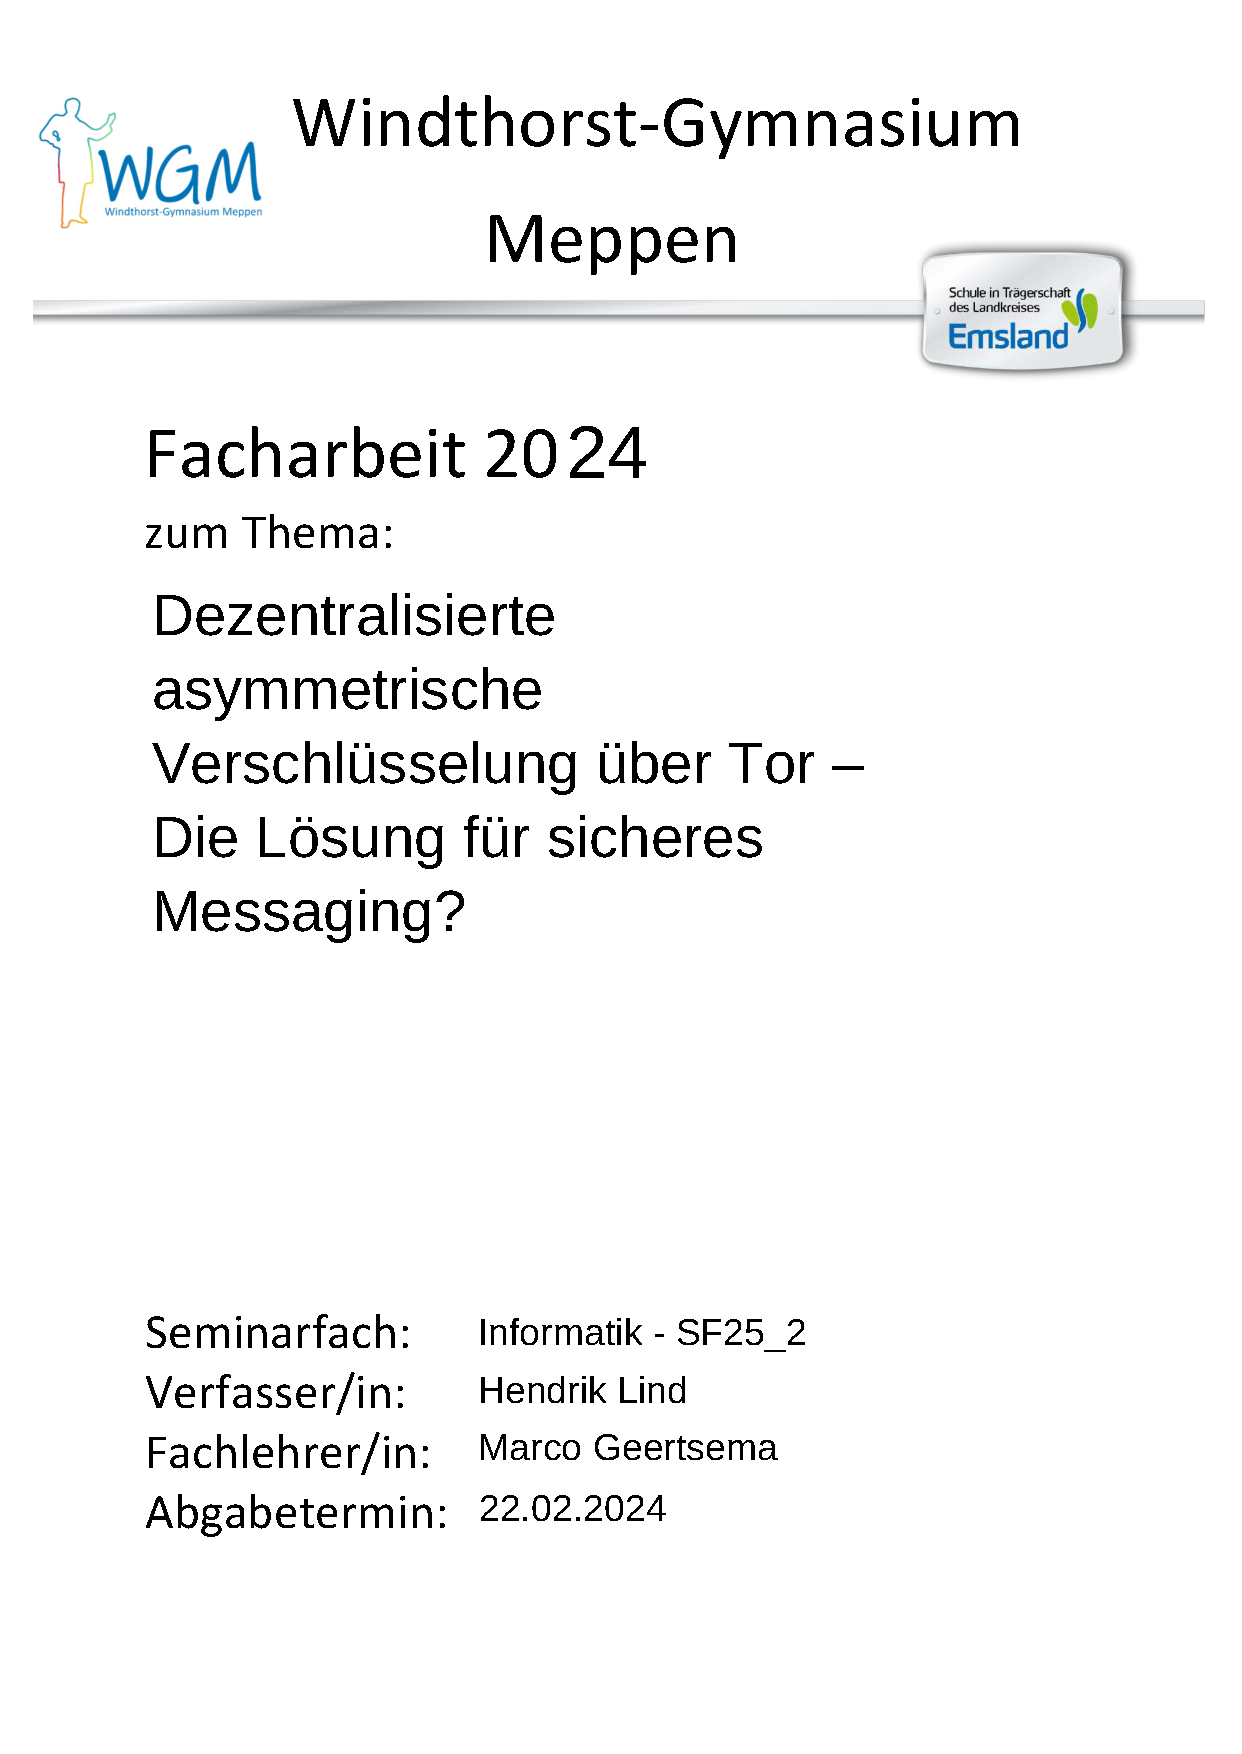
\includepdf[pages=1]{img/signed.pdf}
%% To add this template to the main.tex file, just add the command "% To add this template to the main.tex file, just add the command "% To add this template to the main.tex file, just add the command "\include{titlePageSLU} after "\begin{docuemnt}" in the main.tex file


% In this segment, enter the desired data to be shown at the title page
\newcommand{\thesisAuthor}{Firstname Lastname}
\newcommand{\thesisTitle}{Interesting Thesis Title}
\newcommand{\thesisSubTitle}{little bit more descriptive}
\newcommand{\thesisTitleTranslated}{Translated Headline}
\newcommand{\thesisDegree}{Master thesis project}
\newcommand{\university}{Swedish University of Argicultural Science, SLU}
\newcommand{\credits}{30 hp}
\newcommand{\faculty}{Faculty of blablabalba}
\newcommand{\thesisPlaceDate}{Place of puplication, Year}
\newcommand{\company}{Company name}

%------------------------------------------------------------------------------
\begin{titlepage}
\thispagestyle{empty}
\myfont

% Use this line of code if both SLU loggo and company/other institution loggo is desired. The positions are possible to change with the \hspace and \vspace syntax.
\begin{figure} [H]
\vspace{-3cm}
 \centering
\begin{minipage}[t]{.45\linewidth}
  \raggedright
  % Upload and include SLU loggo here:
  \hspace*{-2cm}
\includegraphics[width=\linewidth]{slu_logo_webb.png}
  
\end{minipage}%
  \begin{minipage}[t]{.45\linewidth}
  \vspace{-3.3cm}
 \raggedleft
% Upload and include other loggo here (loggo of wikipedia is used as an example):
 \hspace*{1cm}
\includegraphics[width =0.5\textwidth]{wikilogo.png} \hspace*{-1cm}
 
\end{minipage}
\end{figure}


% If only the logo for SLU is desired, delete "\begin{comment}" and "\end{comment}" to use this line of code:
\begin{comment}
\begin{figure}
\vspace{-3cm}
    \hspace*{-2cm}
\includegraphics[width = 0.3\textwidth]{slu_logo_webb.png}\hspace*{-2cm}
\end{figure}
\end{comment}


% Adds background picture. Delete code if no background picture is wanted.
\begin{tikzpicture}[overlay, remember picture]
\node[anchor=south west, 
      xshift=-0.2cm, 
      yshift=-0.2cm] 
     at (current page.south west)
     {
\includegraphics[width = 1.8\textwidth, height = 9cm]{background.png}}; 
\end{tikzpicture}


\vspace{1cm}
\par
\noindent
\Huge
\textbf{\thesisTitle}
\vspace{0.2cm}
\LARGE
\par
\noindent
- \thesisSubTitle\\
\rule[0.3cm]{\linewidth}{2pt}
\Large

% Delete this line if no translation is desired
\noindent
\textit{\thesisTitleTranslated}

\vspace{2cm}
\noindent
\LARGE
\thesisAuthor\\
\vspace{4 cm}
\small
\par \noindent
\thesisDegree $\cdot$ \credits
\par \noindent
\university
\par \noindent
\faculty
\par \noindent
\company
\par \noindent
\thesisPlaceDate

\end{titlepage}
 after "\begin{docuemnt}" in the main.tex file


% In this segment, enter the desired data to be shown at the title page
\newcommand{\thesisAuthor}{Firstname Lastname}
\newcommand{\thesisTitle}{Interesting Thesis Title}
\newcommand{\thesisSubTitle}{little bit more descriptive}
\newcommand{\thesisTitleTranslated}{Translated Headline}
\newcommand{\thesisDegree}{Master thesis project}
\newcommand{\university}{Swedish University of Argicultural Science, SLU}
\newcommand{\credits}{30 hp}
\newcommand{\faculty}{Faculty of blablabalba}
\newcommand{\thesisPlaceDate}{Place of puplication, Year}
\newcommand{\company}{Company name}

%------------------------------------------------------------------------------
\begin{titlepage}
\thispagestyle{empty}
\myfont

% Use this line of code if both SLU loggo and company/other institution loggo is desired. The positions are possible to change with the \hspace and \vspace syntax.
\begin{figure} [H]
\vspace{-3cm}
 \centering
\begin{minipage}[t]{.45\linewidth}
  \raggedright
  % Upload and include SLU loggo here:
  \hspace*{-2cm}
\includegraphics[width=\linewidth]{slu_logo_webb.png}
  
\end{minipage}%
  \begin{minipage}[t]{.45\linewidth}
  \vspace{-3.3cm}
 \raggedleft
% Upload and include other loggo here (loggo of wikipedia is used as an example):
 \hspace*{1cm}
\includegraphics[width =0.5\textwidth]{wikilogo.png} \hspace*{-1cm}
 
\end{minipage}
\end{figure}


% If only the logo for SLU is desired, delete "\begin{comment}" and "\end{comment}" to use this line of code:
\begin{comment}
\begin{figure}
\vspace{-3cm}
    \hspace*{-2cm}
\includegraphics[width = 0.3\textwidth]{slu_logo_webb.png}\hspace*{-2cm}
\end{figure}
\end{comment}


% Adds background picture. Delete code if no background picture is wanted.
\begin{tikzpicture}[overlay, remember picture]
\node[anchor=south west, 
      xshift=-0.2cm, 
      yshift=-0.2cm] 
     at (current page.south west)
     {
\includegraphics[width = 1.8\textwidth, height = 9cm]{background.png}}; 
\end{tikzpicture}


\vspace{1cm}
\par
\noindent
\Huge
\textbf{\thesisTitle}
\vspace{0.2cm}
\LARGE
\par
\noindent
- \thesisSubTitle\\
\rule[0.3cm]{\linewidth}{2pt}
\Large

% Delete this line if no translation is desired
\noindent
\textit{\thesisTitleTranslated}

\vspace{2cm}
\noindent
\LARGE
\thesisAuthor\\
\vspace{4 cm}
\small
\par \noindent
\thesisDegree $\cdot$ \credits
\par \noindent
\university
\par \noindent
\faculty
\par \noindent
\company
\par \noindent
\thesisPlaceDate

\end{titlepage}
 after "\begin{docuemnt}" in the main.tex file


%------------------------------------------------------------------------------
\begin{titlepage}
\thispagestyle{empty}
% Use this line of code if both SLU loggo and company/other institution loggo is desired. The positions are possible to change with the \hspace and \vspace syntax.
\begin{figure} [H]
\vspace{-2cm}
 \centering
\begin{minipage}[t]{.45\linewidth}
  \raggedright
  % Upload and include SLU loggo here:
  \hspace*{-2cm}
\includegraphics[width=\linewidth]{wgm.png}
  
\end{minipage}%
  \begin{minipage}[t]{.45\linewidth}
  \vspace{-3.3cm}
 \raggedleft
% Upload and include other loggo here (loggo of wikipedia is used as an example):
 \hspace*{2cm}
\includegraphics[width =0.5\textwidth]{enkrypton.png} \hspace*{-1cm}
 
\end{minipage}
\end{figure}

% Adds background picture. Delete code if no background picture is wanted.
\begin{tikzpicture}[overlay, remember picture]
\node[anchor=south west, 
      xshift=-0.2cm, 
      yshift=-0.2cm] 
     at (current page.south west)
     {
\includegraphics[width = 1.8\textwidth, height = 9cm]{background.png}}; 
\end{tikzpicture}


\vspace{1cm}
\par
\noindent
\Huge
\textbf{\Titel}
\vspace{0.2cm}
\LARGE
\par
\noindent
\SubTitel\\
\rule[0.3cm]{\linewidth}{2pt}
\Large

\vspace{2cm}
\noindent
\LARGE
\Author\\
\vspace{4 cm}
\small
\par \noindent
\thesisDegree
\par \noindent
\School
\par \noindent
\faculty
\par \noindent
\thesisPlaceDate

\end{titlepage}
\tableofcontents
\setcounter{page}{0}
\thispagestyle{empty}
\vspace{0.5cm}
\pagebreak


%//cSpell:enable
% LTeX: enabled=true
%\linenumbers{}
%\modulolinenumbers[5]
%CORRECT_START
\section{Einleitung}
%//SECTION Einleitung
%//TODO hier staatskritisch ist falsches wort mir fällt aber das richtige nicht ein
Russland, China, Iran. In all diesen totalitären Staaten herrscht eine starke Zensur \vcite{AmnReport}. Rund 1,7 Milliarden Menschen sind allein in diesen drei Staaten von der Einschränkung der Meinungsfreiheit betroffen.%//!SECTION
Wie können Bürger dieser Staaten ihre Meinung verbreiten und andere Staaten auf staatskritische Probleme aufmerksam machen, ohne sich selbst in Gefahr zu bringen?%//SECTION Problemstellung
\\
%//TODO Hier nochmal nach einer anderen Quelle suchen, die passt nicht 100%ig
\\
Bei herkömmlichen Messengern wie WhatsApp, Signal und Co. benötigt die Außenwelt die Telefonnummern von Bürgern und Journalisten in einem totalitären Staat, um mit ihnen in Kontakt treten zu können. Eine mögliche Gefahr besteht darin, dass sich ein totalitärer Staat als legitimer Empfänger ausgibt, wodurch Bürger und Reporter ihre privaten Telefonnummern an den Staat weitergeben, der dann in der Lage ist, diese Nummern zurückzuverfolgen \vcite{LocPolice}. Genau hier liegt das Problem: Bürger und Reporter können nicht über gewöhnliche Messenger mit der Außenwelt kommunizieren, da der Staat ihre Nummern zurückverfolgen kann, was die Meinungsfreiheit weiter einschränkt und verhindert \vebd.\\
Die zentralisierte Infrastruktur, die von den meisten Messengern wie WhatsApp und Signal genutzt wird, ermöglicht es auch totalitären Staaten wie China, die IP-Adressen von Servern zu blockieren und sie so für Bürger und Journalisten unzugänglich zu machen \vcite{ChinaFirewall,CentralizedWhatsapp}.%//!SECTION
%//SECTION Lösungsvorschlag / Ziel
%//!SECTION
Ein dezentraler, Ende-zu-Ende-verschlüsselter Messenger, der über das Tor-Netzwerk kommuniziert, könnte eine Lösung für diese Probleme darstellen. Ziel dieser Arbeit ist es, diese Lösung auf ihre Sicherheit und Praktikabilität hin zu untersuchen und zu implementieren.\\
%//SECTION E2EE Überleitung zu Kapitel-Auflistung
%//!SECTION
Um ein Verständnis für die Sicherheit dieses Messengers zu erlangen, geht diese Arbeit im zweiten Kapitel auf die asymmetrische Verschlüsselung und die Ende-zu-Ende-Verschlüsselung (E2EE) ein und beschäftigt sich zunächst mit der mathematischen Betrachtung, um anschließend die Sicherheit des Verfahrens beurteilen zu können. Dabei wird nicht auf das Padding-Verfahren der asymmetrischen Verschlüsselung eingegangen. Im dritten Kapitel wird untersucht, ob das Tor-Netzwerk eine mögliche Lösung für das Problem der Anonymität im Internet darstellt und inwieweit es die Nutzer schützt. Das vierte Kapitel beschäftigt sich mit der Definition und der Sicherheit von Dezentralisierung. Im fünften Kapitel wird schließlich die Implementierung des Messengers beschrieben, während im sechsten Kapitel die Nachteile des Messengers und deren Lösungsmöglichkeiten betrachtet werden. Im siebten Kapitel wird ein Fazit gezogen.%CORRECT_END
\section{Asymmetrische Verschlüsselung}
%//SECTION E2EE und asymmetrische Verschlüsselung
Um einen sicheren Nachrichtenaustausch zu gewährleisten, wird in dieser Arbeit die E2EE implementiert. Bei der E2EE wird von dem Sender die Nachricht, bevor sie an den Empfänger geschickt wird, verschlüsselt \vcite{E2EE}. Dazwischenliegende Akteure, wie zum Beispiel Server oder mögliche Angreifer, können demzufolge die Nachricht nicht lesen \vebd. \textbf{Nur} der Empfänger der Nachricht kann diese auch entschlüsseln. Als Ent- und Verschlüsselungsverfahren der Nachrichten wird die asymmetrische Verschlüsselung verwendet \vebd. Diese Arbeit beschränkt sich bei der asymmetrischen Verschlüsselung auf das RSA-Verfahren.
%//!SECTION
\subsection{Grundlagen}
%//SECTION Grundlagen
Grundsätzlich gibt es bei der asymmetrischen Verschlüsselung ein Schlüsselpaar (Keypair), welches aus einem privaten Schlüssel (private key) und einem öffentlichen Schlüssel (public key) besteht \vcite{Rsa-Basics}. Diese beiden Schlüssel hängen mathematisch zusammen, sodass der öffentliche Schlüssel Nachrichten \textbf{nur} verschlüsseln aber nicht entschlüsseln kann \vebd. \textbf{Nur} der zum Schlüsselpaar dazugehörige private Schlüssel ist in der Lage, die verschlüsselte Nachricht wieder zu entschlüsseln (siehe \cref{fig:E2EE}) \vebd.

\begin{figure}[h]
  \centering
  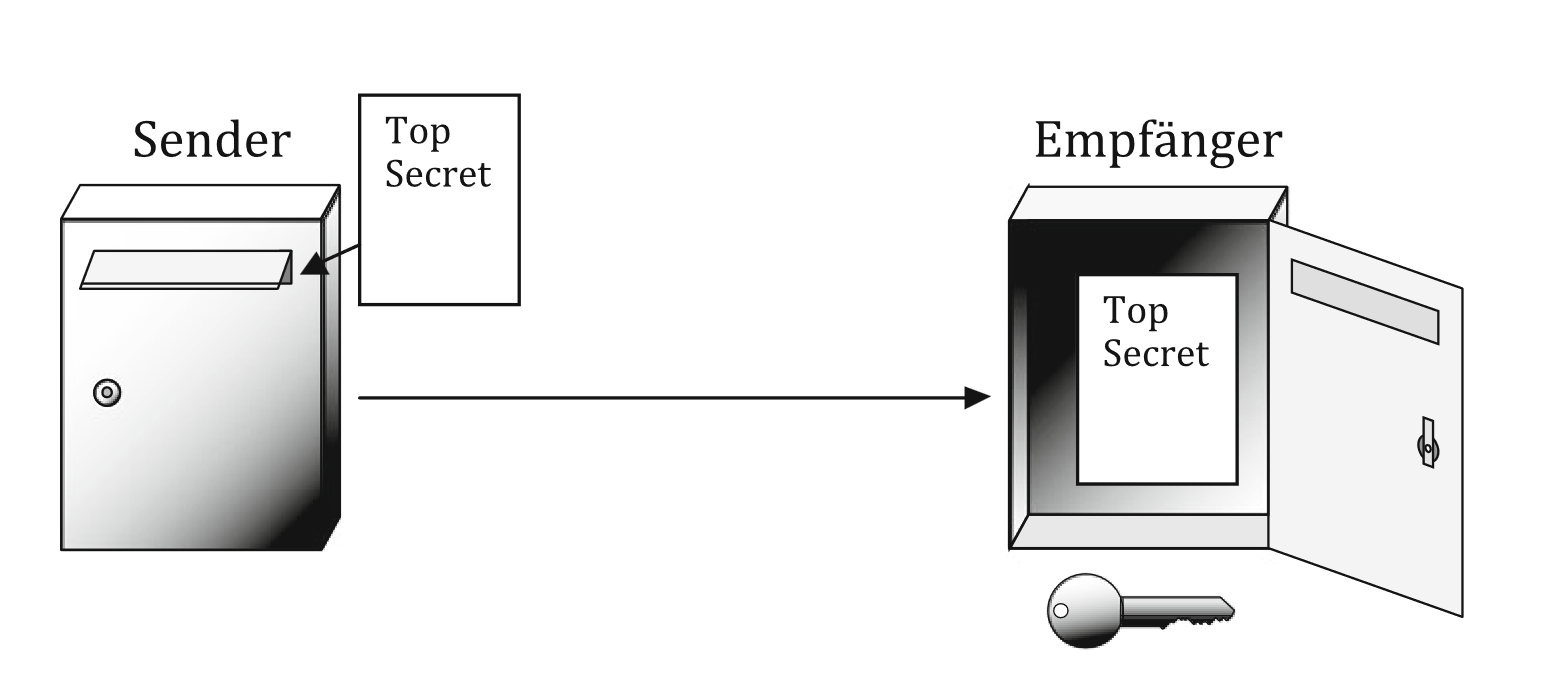
\includegraphics[width=0.75\textwidth]{Briefkasten-asymm.png}
  \caption{Jeder Sender kann mit dem öffentlichen Schlüssel die Nachricht "verschlüsseln" (also eine Nachricht in den Briefkasten werfen), aber nur der Empfänger kann den Briefkasten mit seinem privaten Schlüssel öffnen und somit die Nachricht herausnehmen\vcite{fig:Rsa-Cryptography} \label{fig:E2EE}}
\end{figure}
%//!SECTION

%//SECTION - Mathematische Betrachtung zu RSA
\subsection{Mathematische Betrachtung}
Alle Variablen der folgenden Berechnungen liegen im Bereich $\mathbb{N}$ \vcite{RsaGenCond}. \\
Für die Generierung des Schlüsselpaares benötigen wir zuerst zwei große zufällige Primzahlen, $P$ und $Q$ \vebd. Daraus ergibt sich $n = P * Q$, wobei $P \neq Q$, sodass $P$ bzw. $Q$ nicht durch $\sqrt{n}$ ermittelt werden kann \vebd. Der private Schlüssel besteht aus den Komponenten $\{ n, d \}$ währenddessen der öffentliche Schlüssel aus $\{ n, e \}$ besteht \vcite{RsaVariables}.
%//!SECTION
%//SECTION - Eulersche Phi-Funktion
\subsubsection{Eulersche Phi-Funktion}
Die Eulersche Phi-Funktion spielt eine wichtige Rolle in dem RSA-Verfahren \vcite{TotientFuncMultiplicative}. Grundsätzlich gibt $\phi(x)$ an, wie viele positive teilerfremde Zahlen bis $x$ existieren (bei wie vielen Zahlen der größte gemeinsamer Teiler ($\gcd$) $1$ ist) \vcite{EulersTotientFunction}. Somit ergibt $\phi(6) = 2$  oder bei einer Primzahl $\phi(7) = 7 - 1 = 6$ somit $\phi(x) = x-1$, wenn $x$ eine Primzahl ist, da jede Zahl kleiner als $x$ teilerfremd sein muss \vcite{TotientFuncMultiplicative}.
\begin{equation*}
  \begin{aligned}
    \phi(n) & = \phi(P \cdot Q)                                                \\
    \phi(n) & = \phi(P) \cdot \phi(Q)                                          \\
    \phi(P) & = P -1                                          & \phi(Q) = Q -1 \\
    \phi(n) & = \left(P - 1 \right) \cdot \left( Q - 1\right)
  \end{aligned}
\end{equation*}
%//!SECTION
\subsubsection{Generierung des Schlüsselpaares}
Sowohl der private als auch der öffentliche Schlüssel besteht unter anderem aus folgender Komponente: $n = P \cdot Q$ \vcite{RsaMaths1}.
Für den öffentlichen Schlüssel benötigen wir die Komponente $e$, die zur Verschlüsselung einer Nachricht verwendet wird \vebd. $e$ ist hierbei eine zufällige Zahl, bei welcher folgende Bedingungen gelten \vebd:
\begin{equation*}
  e = \begin{cases}
    1 < e < \phi(n)      \\
    \gcd(e, \phi(n)) = 1 \\
    \text{$e$ kein Teiler von $\phi(n)$}
  \end{cases}
\end{equation*}
Mit der errechneten Komponente $e$, welche Nachrichten verschlüsselt, kann der öffentliche Schlüssel nun an den Sender übermittelt werden.

Um den privaten Schlüssel zu berechnen, benötigen wir die Komponente $d$, welche zur Entschlüsselung verwendet wird \vcite{RsaEncryptionDecryption}.
\begin{equation*}
  \begin{aligned}
    \phi(n)   & = (P-1)(Q-1)     \\
    e \cdot d & = 1 \mod \phi(n)
  \end{aligned}
\end{equation*}

\subsection{Sicherheit}
Um die Sicherheit des RSA-Verfahrens betrachten zu können, müssen wir nun den Ver-/Entschlüsselungsvorgang betrachten.
\begin{equation*}
  \begin{aligned}
    c & = m^e \mod n & \text{Verschlüsselung zu $c$ mit $m$ als Nachricht}    \\
    m & = c^d \mod n & \text{Umkehroperation (Entschlüsslung) von $c$ zu $m$}
  \end{aligned}
\end{equation*}
Um die verschlüsselte Nachricht $c$ zu entschlüsseln, bräuchte ein Angreifer die Komponente des privaten Schlüssels $d$. $d$ ist allerdings mit einem starken Rechenaufwand verbunden, da, wie schon vorher bereits gezeigt, dafür $\phi(n)$ kalkuliert werden müsste. Somit wird eine Primfaktorzerlegung von $n$ benötigt wird \vcite{EulersTotientFunction}. Bei der Verschlüsselung von $m$ zu $c$ liegt eine Trapdoor-Einwegfunktion vor \vcite{RsaTrapdoor}. Das bedeutet, dass es zwar leicht ist $f(x) = i$ zu berechnen (bei RSA: Verschlüsselung), es jedoch unmöglich ist von $i$ auf den Ursprungswert $x$ zu schließen, ohne dass weitere dafür notwendigen Komponente bekannt sind (bei RSA wäre die benötigte Komponente $d$) \vebd.
\begin{figure}[h]
  \centering
  \includesvg[width=0.5\textwidth]{img/Trapdoor_permutation.svg}
  \caption{Die Trapdoor-Einwegfunktion bildlich dargestellt\vcite{fig:TrapdoorPermutation} \label{fig:TrapdoorFunc}}
\end{figure}

Wichtig bei dem RSA-Verfahren ist, dass die Länge von $n$ (die Schlüssellänge) mindestens 3000 Bit betragen sollte, da sonst die Primfaktorzerlegung von $n$ mit modernen Computern möglich sein könnte \vcite{RsaKeyLength}.

%/REVIEW - Ist das wirklich nötig? Oder kann ich mir das sparen? (ja schon)
\subsection{Vergleich zur symmetrischen Verschlüsselung}
Bei der symmetrischen Verschlüsselung wird der gleiche Schlüssel sowohl für die Verschlüsselung als auch für die Entschlüsselung verwendet \vcite{GeneralSymmetricCryptography}.
%/REVIEW - Wirklich padding mit einbeziehen? (meinte er brauch ich nicht)
Im Vergleich zu der asymmetrischen Verschlüsselung, ist die symmetrische Verschlüsselung schneller und keine Beschränkung des Chiffretextes \vcite{RsaAESAnalysis, OpensslRsaMaxLength}. Jedoch muss der Schlüssel der symmetrischen Verschlüsselung sicher an den jeweils anderen Kommunikationspartner übermittelt werden, um Nachrichten zu entschlüsseln \vebd.

\section{Das Tor-Netzwerk}
Die Anonymität des Messengers ist ein weiterer zentraler Aspekt, um die jeweiligen Kommunikationspartner zu schützen. Das Tor-Netzwerk ist hierbei ein möglicher Lösungsansatz, da normalen Routing, wie wir es tagtäglich nutzen, der Client kommuniziert  direkt mit dem Zielserver, somit der Zielserver die IP-Adresse des Clients einsehen kann \vcite{TCP_IP}.
%//REVIEW für den Satz danach Quelle?
Eine Rückverfolgung der IP-Adresse ist somit möglich \vcite{LocPolice}. Und genau bei diesem Problem setzt das Tor-Netzwerk an. Das Tor-Netzwerk besteht hierbei aus vielen \nodes, welche eingehende Tor-Verbindungen akzeptieren und weiterverarbeiten. Damit ein Client eine Anfrage über das Netzwerk verschicken kann, sucht er zunächst einen Pfad durch das Netzwerk, genannt \circuit \vcite{TorCircuits}. Der \circuit besteht dabei meist aus drei \nodes und ist für 10 Minuten gültig, bis der Client das \circuit erneuert (also einen neuen Pfad "sucht")  \vcite{FAQCircuitLifetime}. Die drei \nodes werden klassifiziert in einer \entryn, einer \relayn und einer \exitn, worüber später Anfragen an die Zielserver geschickt werden können \vebd.
Dabei verschlüsselt der Client verschlüsselt die eigentliche Anfrage mehrmals, hüllt sie also in ein mehrere "Schalen" ein, welche eine \onion bilden, und leitet diese über den \circuit an den Zielserver weiter\vcite{TorDesign}. Anfangs wird die \onion von dem Tor-Client an die \entryn geschickt \vebd. Bei jeder \node, wie der \entryn, wird eine Schale der \onion "geschält" (die \onion also einmal entschlüsselt), welche Informationen zu dem nächsten Knotenpunkt enthält \vcite{TorStructure2}. Die Node leitet nun die um eine Schale "geschälte" \onion an den nächsten Knotenpunkt weiter \vebd.
Sobald die Anfrage bei der \exitn angekommen ist, entfernt diese die letzte "Schale" der Anfrage, welche nun vollständig entschlüsselt ist und an den Zielserver geschickt werden kann \vebd. Dieses Routing-Verfahren ist auch als \textit{Onion-Routing} bekannt \vcite{TorDesign}.

\begin{figure}[h]
  \centering
  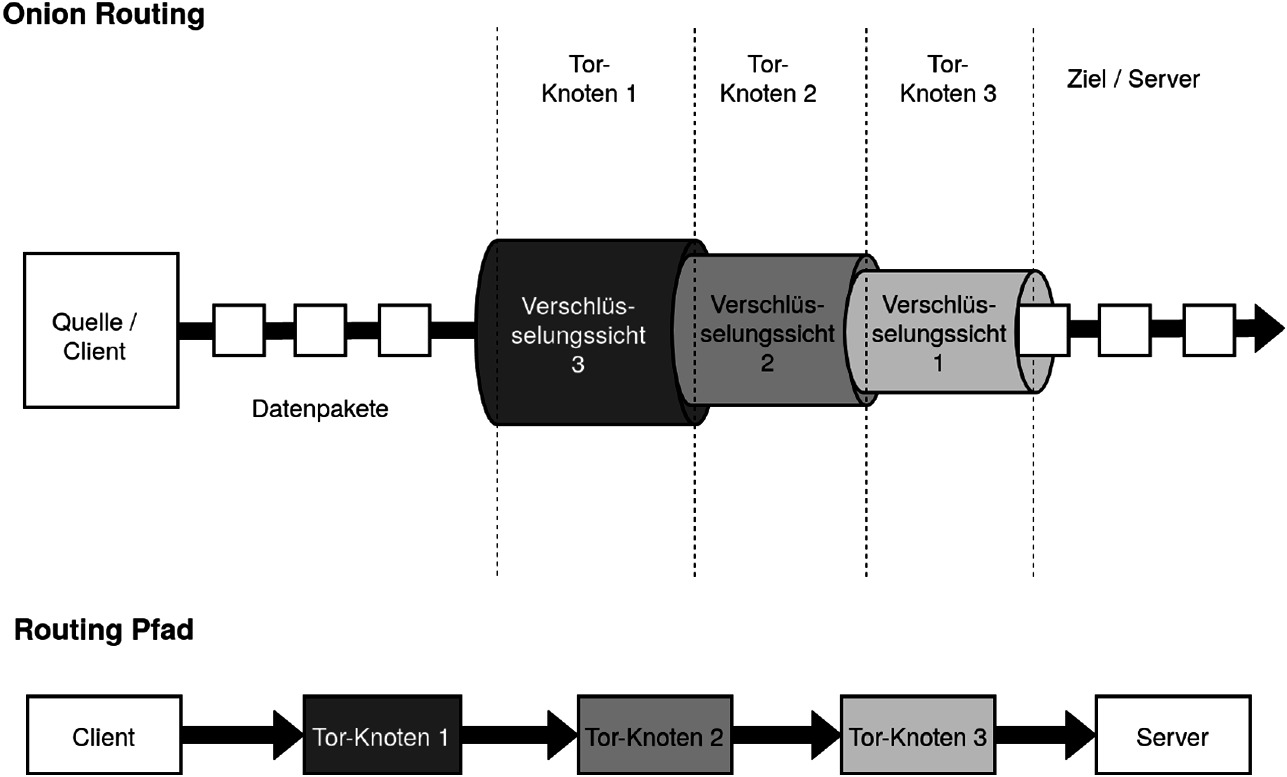
\includegraphics[width=0.65\textwidth]{TorRoutingSimple.png}
  \caption{Das Prinzip des Onion-Routings \vcite{fig:Tor-Structure} \label{fig:TorStructure}}
\end{figure}

%//TODO Checken ob das wirklich in der quelle so steht, sollte eig
\textbf{Nur} die \entryn weiß somit die reale IP-Adresse des Clients und \textbf{nur} die \exitn weiß, an welchen Zielserver die Anfrage geschickt wurde \vcite{TorStructure2}. Dazwischenliegende \nodes, wie die \relayn erkennen nur eine verschlüsselte Anfrage und haben keinerlei Informationen über den eigentlichen Client oder den Zielserver. Die \exitn schickt allerdings die Anfrage ohne Verschlüsselung des Tor-Netzwerkes an den Zielserver, wodurch Informationen der Nutzer ausgelesen werden könnten (wenn die Anfrage nicht über das HTTPS-Protokoll versendet wurde) und zusätzlich die IP-Adresse des Zielservers speichern \vcite{TorExitNodeVulnerability}. Durch Etablieren von \exitns in dem Tor-Netzwerk könnten Angreifer somit die Anonymität des Netzwerkes bzw. der Nutzer gefährden \vebd.

\subsection{Onion Services}
Onion Services sind eine mögliche Lösung für den \exitn-Angriff \vcite{TorOnionServiceTalk}. Diese nicht auf die \exitn angewiesen sind und agieren nur innerhalb des Tor-Netzwerkes mit anderen Tor-Clients und verhalten sich wie normale Tor-Clients \vebd. Onion Services sind nicht über das normale Internet erreichbar, wie die Zielserver im vorherigen Beispiel, sondern nur über das Tor-Netzwerk \vcite{TorOnionService}. Bei Onion Services müssen im Vergleich zu normalen öffentlichen Servern keine Ports geöffnet werden, damit ein Client sich mit dem Server verbinden kann, da der Onion Service direkt mit dem Tor-Netzwerk über ausgehende Verbindungen kommuniziert (auch bekannt als \textit{NAT punching}) und darüber sämtliche Daten geleitet werden \vebd.

%//NOTE bis hier überprüft

\subsubsection{Verbindungsaufbau}
Zunächst generiert der Onion Service ein Schlüsselpaar, bestehend aus einem öffentlichen und einem privaten Schlüssel \vcite{GeeksOnionService}. Unter anderem wird nun aus dem öffentlichen Schlüssel die Adresse des Onion Services generiert und endet mit ".onion" \vebd. Ein Beispiel für eine solche Adresse ist die der Suchmaschine DuckDuckGo: \\
\textit{duckduckgogg42xjoc72x3sjasowoarfbgcmvfimaftt6twagswzczad.onion} \vcite{DuckDuckGoLink}.
%/REVIEW sehr oft gleiche Quelle (L meinte is okay)
Der Onion Service sich nun mit dem Tor-Netzwerk wie ein normaler Client über einen \circuit, welcher aus drei \nodes besteht \vcite{TorOnionService}. Der Service sendet eine Anfrage an das letzte Relay im \circuit, sodass es als \introp dient und etabliert eine Langzeitverbindung jenem (der \circuit erneuert sich also nicht alle 10 Minuten wie bei dem Tor-Client) \vebd. Dieser Vorgang wiederholt sich zweimal, bis der Onion Service drei \introps auf drei verschiedenen \circuits gefunden hat \vebd. Damit andere Clients den Onion Service erreichen können, erstellt der Onion Service einen \textit{Onion Service descriptor}, welcher die Adressen der \introps und Authentifizierungsschlüssel enthält, signiert diesen mit seinem privaten Schlüssel und schickt den \textit{Descriptor} an die Directory Authority \vcite{TorSpecDerivingKeys, TorSpecDirectoryInf}. Die Directory Authority ist ein Server, welcher Informationen über das Tor-Netzwerk, wie zum Beispiel die des Onion Services, speichert und verteilt \vcite{TorDirectoryAuthority}. Im Sinne dieser Arbeit, hat der Onion Service sich nun von Person A mit dem Tor-Netzwerk verbunden, jedoch braucht es noch Person B, welche sich über ihren Tor-Client mit dem Onion Service der Person B verbindet. Damit der Tor-Client von Person A sich allerdings verbinden kann, fragt der Client nun die Directory Authority an den signierten \textit{Descriptor} des Onion Services von Person B an den Client zu schicken \vcite{TorStructure}. Der Client besitzt nun die Adressen der \introps und die Signatur des \textit{Descriptors}, sodass dieser mit dem öffentlichen Schlüssel der Onion Adresse die Signatur überprüfen kann \vebd. Der Client generiert nun 20 zufällige Bytes (Secret) und schickt diese an eine zufällig ausgewählte \relayn, welche nun als \renp dient \vcite{TorSpecRendezvous}. Das Secret wird von dem Client auch an eine von den \introps geschickt, sodass der Onion Service mit dem gleichen Secret eine Verbindung zu dem \renp aufbauen kann \vcite{TorSpecIntroP}. Der \renp leitet, wenn der Client und der Onion Service über deren \circuits miteinander verbunden sind, die Nachrichten zwischen den beiden weiter \vcite{TorSpecRendezvous}. Der Client und der Onion Service kommunizieren nun also nur über das Tor-Netzwerk miteinander und sind nicht mehr auf die \exitn angewiesen.

\subsection{Sicherheit}
%//TODO Nochmal Studio durchlesen, ist noch nicht schlüssig
%//TODO Angriff wurde schon von Tor gefixt, benutze OnionServiceFingerprinting
%//TODO Clearnet erklären
In der Sicherheitsbetrachtung beziehe ich mich ausschließlich auf die Verbindung zwischen Onion Services und Tor-Clients (also nicht zwischen Tor-Client und \exitn).

Das Tor-Netzwerk in Verbindung mit den Onion Services liefert, wie bereits erläutert, durch \circuits und \renp eine hohe Anonymität. Im Gegenzug sorgt die hohe Anonymität, welche durch die vielen \nodes und durch mehrfache Verschlüsselungen erreicht wird, auch dazu, dass das Tor-Netzwerk um das 120-fache langsamer ist im Vergleich zum normalen Routing \vcite{TorPerformance}.
Das Tor-Netzwerk ist praktisch unmöglich in der Praxis zu blockieren, da über 6.500 verschiedene \nodes existieren und es somit keinen zentralen Hauptserver gibt, von welchem das Tor-Netzwerk abhängig ist \footnote{Es ist zwar möglich die IP-Adressen jeglicher \relayns zu blockieren, jedoch ist dies durch Pluggable Transports umgänglich \vcite{PluggableTransports}} \vcite{DeanonymizingTorBook}.
Theoretisch ist eine Deanonymisierung eines Onion Services möglich, wenn der ISP (Internet Service Provider, also z.B. Telekom, EWE, etc.) eingehende und ausgehende Verbindungen zwischen Client und Onion Service bzw. zu deren \relayn aufzeichnet und diese mithilfe von Machine Learning analysiert \vcite{OnionServiceFingerprinting}. Dabei war die Umsetzung der theoretischen Grundlage bis jetzt mit idealisierten Bedingungen erfolgreich, jedoch braucht es noch weiterer Studien, um die möglichen Gefahren dieses Algorithmus einzustufen \vebd. Dabei könnten, wenn die deutsche, amerikanische und die französische Regierung zusammenarbeiten, 78,34 \% der \circuits deanonymisieren \vebd.
%//FIXME - Hier is irgend nen Kasus Fehler
Dieses Szenario erscheint jedoch unrealistisch, da Bürger in Deutschland, in den USA und in Frankreich ein Recht auf Meinungsfreiheit besitzen und höchstwahrscheinlich keine Deanonymisierungsangriff starten, um die Privatsphäre zum Beispiel von Whistleblowern zu schützen  \vcite{AmnReport,ROG-USA}.
%//TODO Später nochmal hier drauf eingehen, ist unrealistisch, dass die Regierungen zusammenarbeiten, um Meinungsfreiheit und Whistleblower unterdrücken.


\section{Dezentralisierung}
Mit den vorgeschlagenen Konzepten ist der Messenger imstande anonym (durch das Tor-Netzwerk und Onion Services) und sicher (durch asymmetrische Verschlüsselung) zu kommunizieren, jedoch wurde die Infrastruktur des Messengers noch nicht behandelt. Dafür ist die Betrachtung und Abwägung eines zentrales bzw. dezentrales Netzwerkes notwendig. \\
Ein zentrales Netzwerk, zum Beispiel das Netzwerk von WhatsApp oder Signal, besteht aus einem Hauptserver, welcher Daten verarbeitet und mit welchem sich Clients verbinden können \vcite{WhatsappCentralized,SignalCentralized, CentralizedDefinition}.
%//REVIEW - Dass der Client vertrauen muss ist angegeben, aber nicht dass er es nicht überprüfen kann
Der Client muss bei dieser Netzwerkstruktur dem Hauptserver "vertrauen" und kann nicht überprüfen, ob der Server von einem Hacker kompromittiert wurde \vcite{MessagingNetwork}. Dezentrale Netzwerke bestehen hingegen aus mehreren Servern, auf welche Rechenoperationen und oder Daten aufgeteilt werden \vcite{DecentralizedDefinition}.


\subsection{Sicherheit}
%//REVIEW - Muss ich hier wirklich noch sagen warum durch Kompromittierung Daten ausgelesen werden können? Bzw. die zentrale Angriffsfläche ist doch logisch oder?
Im Beispiel eines Messengers bietet ein zentrales Netzwerk den Hauptserver als mögliche Angriffsfläche an, sodass diese entweder durch DDoS-Angriffe außer Betrieb gesetzt werden kann oder durch Kompromittierung des Servers sowohl der Empfänger als auch der Sender der Nachrichten ausgelesen werden kann (in Form von Onion-Adressen)\vcite{BSI-DDoS}.
%//TODO - Satz bisschen scuffed, ausschalten nicht das richtige Wort.
Ein dezentrales Netzwerk mit einer Peer-to-Peer-Architektur\footnote{Peer-to-Peer bedeutet, dass jeder Knotenpunkt im Netzwerk sowohl Client als auch Server sein kann, welche bidirektional kommunizieren \vcite{PeerToPeerDef}} hat hingegen eine größere Angriffsfläche, wodurch mehrere Knotenpunkte des Netzwerkes kompromittiert werden müssen, um das Netzwerk ausschalten zu können \vcite{GeeksCenralizeDecentralized}.
%//REVIEW - Hier gibt es irgendwie keine Quellen, maybe einfach logisch?
Am Beispiel des Messengers, sollten nur Gesprächsteilnehmer Teil des Netzwerkes sein, um zu verhindern, dass ein Angreifer durch einfaches Beitreten des Netzwerkes die Onion-Adressen der Gesprächsteilnehmer auslesen kann.


\section{Umsetzung des Messengers}
Um den Messenger umzusetzen, müssen zunächst die Anforderung des Messengers bekannt sein. Somit sollten folgende Kriterien erfüllt sein:
\begin{description}
  \item[Einfache Bedienung und Installation] - Möglichst wenig Kenntnisse über Computer sollten benötigt werden, um diesen Messenger zu installieren und zu benutzen
  \item[Peer-to-Peer-Verbindung] - Nur über eine direkte Verbindung miteinander kommunizieren
  \item[Anonymität] - Kommunikation über das Tor-Netzwerk
  \item[Sicherheit] - Verschlüsseltes Speichern von Nachrichten und Schlüsselpaaren, um Auslesen der Daten (z.B. durch totalitäre Staaten) zu verhindern
  \item[E2EE] - Verschlüsselung der Nachrichten und Verifikation des Kommunikationspartners
\end{description}
Damit der Nutzer keine Konsole verwenden muss, um den Messenger zu benutzen, habe ich eine Desktopapplikation mit Rust und Tauri entwickelt. Durch Tauri sind keine weiteren Installationen von Bibliotheken nötig, wodurch eine einfache Installation gegeben ist. %//REVIEW - Hier Quelle? Weil ich habs ja programmiert sind ja keine weiteren Installationen dafür nötig
Zudem kann die Applikation für Windows, Linux und (theoretisch) MacOS kompiliert werden \vcite{RustCompile}. Rust bietet eine hohe Performance und ist Memory Safe, wodurch viele Sicherheitslücken, wie Buffer Overflows, verhindert werden können \vcite{RustSecurity}. Das Tauri-Framework bietet hierbei zwischen User Interface (UI), welches ich in Typescript und React programmiert habe, und Rust-Backend eine Schnittstelle, um Daten (\textit{payloads}) zwischen Frontend und Backend zu versenden \vcite{TauriPayloads}. Ich werde in dieser Umsetzung nicht auf den Quellcode des Frontends eingehen, da dieser nur für das UI zuständig ist und keine weiteren Funktionalitäten bietet.
\begin{comment}
\subsection{Bibliotheken - Übersicht}
Der Messenger ist in verschiedene Bibliotheken nach ihren Funktionen aufgeteilt worden:
\subsubsection*{encryption}
Diese Bibliothek ermöglicht es, Nachrichten zu verschlüsseln und zu entschlüsseln, wobei das RSA-Verfahren benutzt wird. Zudem können durch diese Bibliothek Schlüsselpaare in Text umgewandelt und wieder zurückgewandelt werden.
\subsubsection*{messaging}
Eine Kommunikation zwischen Messengern wird durch diese Bibliothek ermöglicht. Sie führt den Client und den Server zusammen und ist für den Versand bzw. Empfang von Nachrichten zuständig
\subsubsection*{payloads}
Eine Kollektion an verschiedenen Netzwerkpackets und \textit{paylods}, welche unter anderem für die Kommunikation zwischen Messengern verwendet werden.
\subsubsection*{secure-storage}
Durch diese Bibliothek können beliebige Structs symmetrisch verschlüsselt, gespeichert und wieder geladen / entschlüsselt werden.
\subsubsection*{shared}
Beinhaltet gemeinsame Funktionen und Konstanten, zum Bespiel die Tor-Proxy-Konfiguration.
\subsubsection*{storage-internal}
Die Implementierung der \textit{secure-storage} Bibliothek.
%//TODO gehändelt ist richtig scheiße
\subsubsection*{tor-proxy}
Der Tor-Proxy wird durch diese Bibliothek gestartet, sodass ein Onion Service im Tor-Netzwerk etabliert werden kann. \\

Da die Messenger mit einer Peer-to-Peer-Verbindung miteinander verbunden sind, muss jeder Messenger in der Lage sein sowohl als Client als auch als Server (in Form eines Onion Services) zu agieren.
\end{comment}

\subsection{Peer-to-Peer-Verbindung}
Damit Messenger in der Lage sind, sowohl als Client als auch als Server zu fungieren, startet jeder Messenger einen HTTP-Server, welcher einen HTTP-Endpunkt anbietet (in diesem Messenger \textit{/ws/}), mit welchem eine Websocket\footnote{%//TODO Hier richtig zitieren
  Ein Protokoll für bidirektionale Kommunikation zwischen Server und Client über HTTP \vcite{WebsocketDef}}-Verbindung durch Clients aufgebaut werden kann. Der Server ist hierbei also in der Lage sowohl Packets %//TODO -  Packets noch erklären?
zu empfangen als auch zu senden.
\begin{minted}[breaklines]{rust}
HttpServer::new(|| {
    return App::new()
        // Return the default message to tell other clients that this server is actually alive
        .service(hello)
        // The websocket endpoint
        .route("/ws/", web::get().to(ws_index));
})
// Bind just to localhost and run
.bind(("127.0.0.1", CONFIG.service_port()))?
.run()
.await?;
\end{minted}

Analog dazu besitzt jeder Messenger auch einen Websocket-Client, welcher sich im direkten Weg (über das Tor-Netzwerk) mit den anderen Messengern verbinden kann. Der Verbindungsaufbau zu anderen Messengern sieht wie folgt aus:
\begin{minted}[breaklines]{rust}
/// `onion_hostname` is the onion address of the other messenger to connect to
pub async fn new(onion_hostname: &str) -> Result<Self> {
  // [...]
  let connect_host = onion_hostname.to_string();

  //[...]

  // The address which is used to connect to the websocket
  let onion_addr = format!("ws://{}.onion/ws/", connect_host);

  debug!("[CLIENT] Creating proxy...");

  // Creating the Socks5Proxy client which is used to connect to the tor network
  let proxy = SocksProxy::new()?;
  debug!("[CLIENT] Connecting Proxy...");
  let mut onion_addr = Url::parse(&onion_addr)?;
  onion_addr
      .set_scheme("ws")
      .or(Err(anyhow!("[CLIENT] Could not set scheme")))?;

  // Connecting to the destination host using the proxyy
  let sock = proxy.connect(&onion_addr).await?;

  //[...]
  // Connecting to the websocket with the client
  let (ws_stream, _) = tokio_tungstenite::client_async(&onion_addr, sock).await?;

  // [...]
}
\end{minted}
Damit zwei Nutzer über den Messenger Nachrichten versenden können, muss ein Messenger die Rolle als Client und der ander als Server übernehmen. Dabei nimmt der Messenger, welcher die Verbindung zu einem anderen Messenger initiiert hat, die Rolle als Clients ein und der andere Messenger die Rolle als Server. Dadurch, dass jeder Messenger sowohl Client als auch Server sein kann, müssen empfangene Nachrichten von Client und Server zusammengeführt und an das Frontend übermittelt werden, welches in der Bibliothek \textit{messaging} implementiert ist:
\begin{minted}{rust}
/// A Manager which holds the connections by receiver name
pub struct MessagingManager {
  /// The connections by receiver name
  pub(crate) connections: Arc<RwLock<HashMap<String, Connection>>>,
}

/// A generalized connection struct that can be used for both the client and the server
#[derive(Debug, Clone)]
pub struct Connection {
    pub(super) info: Arc<RwLock<ConnInfo>>,
    read_thread: Arc<Option<ConnectionReadThread>>,
    pub(crate) self_verified: Arc<RwLock<bool>>,
    pub(crate) verified: Arc<RwLock<bool>>,
    pub(super) receiver_host: String,

    notifier_ready_tx: Sender<()>,
    notifier_ready_rx: Receiver<()>,
}
\end{minted}
Der \textit{MessagingManager} hält sowohl Verbindungen von Client zu Server und Server zu Client in einem generellen Konstrukt, der \textit{Connection} fest. Diese \textit{Connection}s werden in einer \textit{HashMap} gespeichert. Der \textit{MessagingManager} bietet eine Schnittstelle für das Frontend, um Nachrichten zu senden und zu empfangen.
\begin{figure}[h]
  \centering
  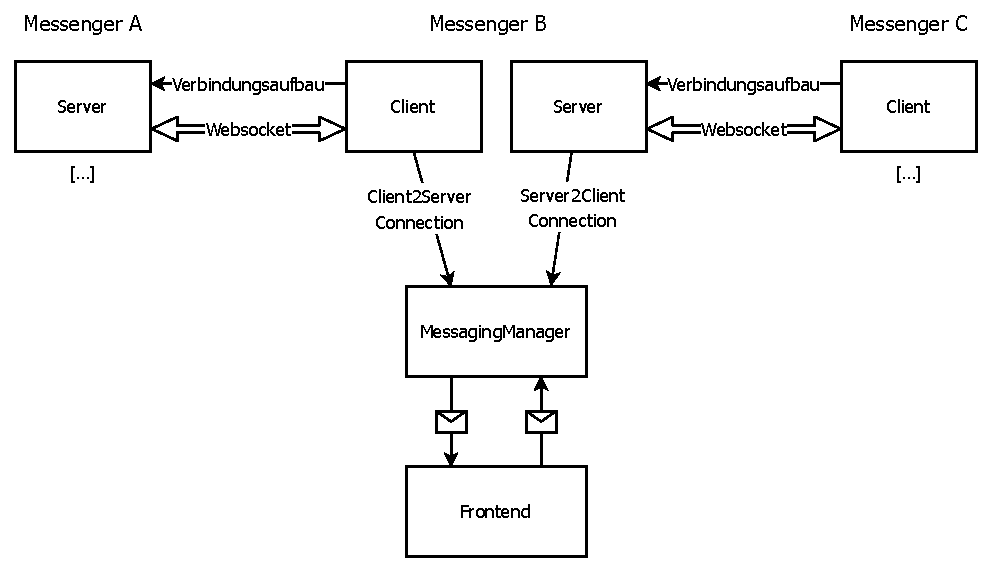
\includegraphics[width=\textwidth]{diagrams/messaging_messenger.pdf}
  \caption{Mögliches Beispiel für Messenger B, welcher eine Verbindung zu Messenger A aufgebaut hat, und Messenger C, welcher mit Messenger B verbunden ist \label{fig:MessagingMessenger}}
\end{figure}
Wenn in diesem Beispiel das Frontend eine Nachricht an Messenger A senden möchte, würde diese Nachricht zunächst an den \textit{MessagingManager} geschickt, welcher diese verschlüsselte Nachricht an den dazugehörigen Client leitet. Der Client leitet nun die Nachricht über den Websocket an den Server des Messengers A weiter.


\subsection{Tor-Netzwerk}
Eine mögliche Lösung für das Kriterium der Anonymität besteht im Tor-Netzwerk. Eine Verbindung muss also zum Tor-Netzwerk aufgebaut werden, welches durch die \textit{tor-proxy} Bibliothek geschieht.
Der HTTP-Server wird auch durch den Tor-Proxy in das Tor-Netzwerk eingebunden. Damit der Tor-Proxy sich jedoch mit dem Tor-Netzwerk verbinden kann, wird eine Konfigurationsdatei benötigt, welche durch die \textit{tor-proxy} Bibliothek erstellt wird:
\begin{minted}{rust}
/// Converts the configuration to a `torrc` file format
async fn to_text(&self) -> Result<String> {
    let data = PathBuf::from(self.data_dir());

    let geo_ip = data.clone().join("geoip");
    let geo_ip6 = data.clone().join("geoip6");

    #[allow(unused_mut)]
    let mut config = format!(
        "SocksPort {}
HiddenServiceDir \"{}\"
HiddenServicePort 80 {}
DataDirectory \"{}\"
GeoIPFile \"{}\"
GeoIPv6File \"{}\"",
        self.get_socks_host(),
        self.service_dir().to_string_lossy().replace("\\", "/"),
        self.get_hidden_service_host(),
        self.data_dir().to_string_lossy().replace("\\", "/"),
        geo_ip.to_string_lossy().replace("\\", "/"),
        geo_ip6.to_string_lossy().replace("\\", "/"),
    );

    //[...]

    Ok(config)
}
\end{minted}
Eingehende Verbindung zum Onion Service dieses Messengers werden also nun zum Port des HTTP-Servers weitergeleitet. Nun muss der Tor-Proxy nur noch gestartet werden:
\begin{minted}{rust}
let mut child = Command::new(TOR_BINARY_PATH.clone());
child.args(["-f", &get_torrc().to_string_lossy()]);
child.current_dir(TOR_BINARY_PATH.parent().unwrap());
child.stdout(Stdio::piped());
child.stderr(Stdio::piped());
//[...]
let child = child.spawn()?;
\end{minted}

Der Messenger ist jetzt mit dem Tor-Netzwerk verbunden und der HTTP-Server ist über den Onion Service erreichbar. Andere Messenger können sich nun anonym über das Tor-Netzwerk mit diesem Messenger verbinden.
\subsection{Sicherheit}
Ein Datenspeicher, welcher symmetrisch verschlüsselt ist, wird durch die Bibliothek \textit{secure-storage} implementiert. Mit dieser Bibliothek lassen sich beliebige \textit{Structs} in Text umwandeln und verschlüsseln bzw. auslesen und entschlüsseln. Die \textit{storage-internal} Bibliothek benutzt hierbei die Methoden der \textit{secure-storage} Bibliothek und dient als Wrapper, um die Daten auf der Festplatte zu speichern und wieder auszulesen. Der Datenspeicher enthält hierbei eine \textit{HashMap}, welche als Schlüssel die Onion Adresse anderen Messengers und als Wert die Chatinformationen enthält. Die Chatinformationen sind zum Beispiel gesendete oder versendete Nachrichten, Schlüsselpaare und öffentliche Schlüssel.
\begin{minted}[breaklines]{rust}
#[derive(Clone, Debug, Serialize, Deserialize, Zeroize, ZeroizeOnDrop)]
pub struct StorageChat {
  /// All messages sent to this receiver or received from this receiver
  pub messages: Vec<ChatMessage>,
  //[...]

  /// The public key which is used to encrypt messages when being sent to the receiver [...]
  #[zeroize(skip)]
  pub rec_pub_key: Option<PublicKey>,
  /// Private key of this messenger used to decrypt the messages that are being received [...]
  pub priv_key: PrivateKey,
}
\end{minted}
Der \textit{StorageChat} enthält die Nachrichten, welche an den Empfänger gesendet oder von diesem empfangen wurden (\textit{messages}), den öffentlichen Schlüssel des Kommunikationspartner (\textit{rec\_pub\_key}) und den privaten Schlüssel des Messengers \textit{priv\_key}.
%//REVIEW - Kann ich das so sagen?
Um die Daten des Nutzers vor weiteren möglichen Angriffen zu schützen, verwende ich die Bibliothek \textit{zeroize}, welche sensible Daten (wie private Schlüssel) aus dem Arbeitsspeicher löscht (Zeroisation) \vcite{Zeroization}. Zudem ist es durch die symmetrische Verschlüsselung des Datenspeichers für Angreifer nicht möglich (sofern die Applikation geschlossen ist), private Schlüssel oder Chatverläufe auszulesen, wodurch die Privatsphäre der Nutzer geschützt wird.

\subsection{Ende-zu-Ende-Verschlüsselung}
Das letzte Kriterium, welches der Messenger nun erfüllen muss, ist die Ende-zu-Ende-Verschlüsselung. Dafür muss zuerst die Identität des anderen Kommunikationspartners verifiziert werden.
\subsubsection{Identity verification}
Um das Konzept der E2EE umzusetzen, muss der Sender einer Nachricht sicher sein, dass der Empfänger tatsächlich der ist, für den er sich ausgibt, wofür die \textit{Identity verification} stattfindet. Im Rahmen der Erklärung gehen wir nun davon aus, dass Messenger A an Messenger B eine Nachricht senden möchte. Messenger A wäre in diesem Fall der Client und Messenger B der Server.
Messenger A und Messenger B generieren anfangs (wenn noch nicht vorhanden) private Schlüssel und erstellen ein neues \textit{StorageChat}-Konstrukt, in welchem die privaten Schlüssel gespeichert werden.
Damit sowohl Client als auch Server sicher sein können, dass der Kommunikationspartner tatsächlich der ist, für den er sich ausgibt, wird zunächst von dem Client ein \identity-Packet versendet.
Dies besteht aus dem eigenen Hostname, der Signatur des Hostnames und dem Zielhostname (durch den privaten Schlüssel des Chats signiert) und den öffentlichen Schlüssel des Schlüsselpaares (vom Chat). Das Identitätspacket wird also folgendermaßen generiert:
\begin{minted}{rust}
async fn identity(receiver: &str) -> Result<Self> {
  // Get the own hostname
  let own_hostname = get_service_hostname(true)
  .await?
  .ok_or(anyhow!("Could not get own hostname"))?;

  // Get the private key for the receiver (used to decrypt messages)
  let priv_key = StorageManager::get_or_create_private_key(receiver).await?;
  let pub_key = priv_key.clone().try_into()?;

  // Creating a signature for the receiver with the hostname
  let keypair = PKey::from_rsa(priv_key.0)?;
  let mut signer = Signer::new(*DIGEST, &keypair)?;

  signer.update((own_hostname.clone() + receiver).as_bytes())?;
  let signature = signer.sign_to_vec()?;

  // Return the identity packet
  Ok(C2SPacket::SetIdentity(Identity {
    hostname: own_hostname,
    signature,
    pub_key
  }))
}
\end{minted}
Ein wichtiges Detail ist hierbei die Signatur des \identity-Packets. Sie besteht sowohl aus dem eigenen Hostname als auch dem Ziel des Hostnames, um zu verhindern, dass ein Angreifer das \identity-Packet abfängt und sich damit als Messenger des dazugehörigen Packets ausgibt.
Nachdem der Server das Packet empfangen hat, überprüft er dieses. Dazu ruft dieser den öffentlichen Schlüssel des Kommunikationspartners auf, und verifiziert mit diesem die Signatur des \identity-Packets:
\begin{minted}[breaklines]{rust}
async fn verify(&self) -> Result<()> {
  let Identity {  hostname: remote_host, pub_key, signature} = self;
  // Get the own hostname
  let own_hostname = get_service_hostname(!remote_host.ends_with("-dev-client"))
      .await?
      .ok_or(anyhow!("Could not get own hostname"))?;


  debug!("Reading to verify...");
  // Check if there is a public key for the given receiver
  let local_pub_key = STORAGE.read().await.get_data(|e| {
      let key = e.chats.get(remote_host)
          .and_then(|e| e.rec_pub_key.clone());

      Ok(key)
  }).await?;

  debug!("Done");

  // If there is a public key, verify the signature
  if let Some(local_pub_key) = local_pub_key {
      info!("Verifying for hostname: {:?}", remote_host);
      let keypair = PKey::from_rsa(local_pub_key.0)?;
      let mut verifier = Verifier::new(*DIGEST, &keypair)?;

      // Verify the signature with the public key
      verifier.update((remote_host.to_string() + &own_hostname).as_bytes())?;
      let is_valid = verifier.verify(&signature)?;

      if !is_valid {
          warn!("[INVALID_SIGNATURE] Wrong signature was given! This may be an attack!");
          return Err(anyhow!("Wrong signature was given! This may be an attack!"));
      }

      Ok(())
  } else {
      // Adding public key to storage because it does  not exist
      info!("No chat with hostname '{}' yet. Adding new receiver...", remote_host);
      STORAGE.read().await.modify_storage_data(|e| {
          let res = e.chats.entry(remote_host.clone())
              .or_insert_with(|| StorageChat::new(&remote_host));

          res.rec_pub_key = Some(pub_key.clone());

          Ok(())
      }).await?;
      debug!("Done.");

      Ok(())
  }
}
\end{minted}
Falls die Identität valide ist, übersendet der Server seine Identität an den Client. Der gleiche Vorgang der Validation findet nun auch auf dem Client statt. Wenn dieser die \identity als valide betrachtet, ist eine sichere Verbindung zwischen Client und Server aufgebaut.
\subsection{Nachrichten versenden}
Gehen wir davon aus, dass der Client an den Server über die gesicherte Verbindung eine Nachricht versenden möchte. Dazu ruft er zunächst den öffentlichen Schlüssel des Empfängers aus dem Datenspeicher ab und verschlüsselt die Nachricht mit dem RSA-Verfahren. Anschließend übersendet er die verschlüsselte Nachricht an den Server.
\begin{minted}[breaklines]{rust}
/// Sends a message to the receiver with the given date and msg, internal function
async fn inner_send(&self, msg: &str, date: u128) -> Result<()> {
  let raw = msg.as_bytes().to_vec();

  let tmp = self.receiver_host.clone();
  debug!("Reading public key for {}...", tmp);

  // Firstly we need to get the public key of the receiver
  let pub_key = STORAGE
    .read()
    .await
    .get_data(|e| {
      e.chats
        .get(&tmp)
        .and_then(|e| e.rec_pub_key.clone())
        .ok_or(anyhow!("The pub key was empty (should never happen)"))
    })
    .await?;

  debug!("Sending");
  // And encrypt the message
  let bin = pub_key.encrypt(&raw)?;

  // And send it to the receiver, if we are the client, send a client packet if not, server packet
  match &*self.info.read().await {
    ConnInfo::Client(c) => {
      debug!("Client msg");
      let packet = C2SPacket::Message((date, bin));
      c.feed_packet(packet).await?;
    }
    ConnInfo::Server((_, s)) => {
      debug!("Server msg");
      let packet = S2CPacket::Message((date, bin));

      s.send(packet).await?;
    }
  };

  Ok(())
}
\end{minted}
Der Server empfängt über die Websocket-Verbindung die verschlüsselte Nachricht des Clients und entschlüsselt diese anschließend mit dem privaten Schlüssel des Chats. Somit wurde die Nachricht empfangen, entschlüsselt und wird nun an das Frontend übermittelt, sodass diese angezeigt werden kann. Nutzer können nun sicher und anonym miteinander kommunizieren.
\section{Nachteile und Lösungsmöglichkeiten}
Der Messenger bietet zwar hohe Anonymität und Sicherheit, jedoch ist es unerlässlich auch die Nachteile des Messengers und deren Lösungsmöglichkeiten zu betrachten. Durch die Struktur des Tor-Netzwerkes können Datenmengen um das 120-fache langsamer übermittelt werden, welches bei einfachen Textnachrichten nicht auffallen mag, bei größeren Datenmengen, wie zum Beispiel Bildern, jedoch ein Problem darstellen könnte \vcite{TorPerformance}. Dadurch, dass der Client eine Websocket-Verbindung mit dem Onion Service aufbaut, herrscht hier ein \textit{long-term-circuit}, wodurch der \circuit zwischen Onion Service und Client nicht erneuert wird, somit für Angriffe anfälliger sein könnte \vcite{FAQCircuitLifetime}. Zusätzlich ist die Nachrichtenlänge durch das Padding der asymmetrischen Verschlüsselung begrenzt \vcite{OpensslRsaMaxLength}. %//REVIEW - Ich hab die Studie hierbei angewendet, ist das okay?
Eine hybride Verschlüsselung, also eine Kombination aus asymmetrischer und symmetrischer Verschlüsselung, könnte eine mögliche Lösung für die limitierte Nachrichtenlänge sein \vcite{HybridEncryption}. Dabei generiert bereits bei dem Verbindungsaufbau der Server einen zufälligen symmetrischen Schlüssel \vebd. Dieser wird mit dem öffentlichen Schlüssel des Clients verschlüsselt und an den Client übermittelt, welcher diesen entschlüsselt und abspeichert, sodass sowohl Server als auch Client den gleichen symmetrischen Schlüssel teilen \vebd.
%//REVIEW - Nochmal zitieren warum schnell und keine Nachrichtenlängenbegrenzung?
Somit werden die Vorteile der symmetrischen Verschlüsselung (schnell und keine Nachrichtenlängenbegrenzung) mit den Vorteilen der asymmetrischen Verschlüsselung (sicherer Austausch von Schlüsseln) kombiniert \vcite{HybridTechnopedia}. Aufgrund der Infrastruktur dieses Messengers, müssen beide Kommunikationspartner den Messenger geöffnet haben, damit diese miteinander kommunizieren können (der Onion Service wird nur durch Öffnen des Messengers gestartet).

\section{Fazit}
In der heutigen Gesellschaft wird die Meinungsfreiheit der Bürger, welche in einem totalitären Staat leben, immer wichtiger. Das Tor-Netzwerk bietet hierbei eine Möglichkeit, anonym und sicher über Onion Services miteinander zu kommunizieren. Mit dem Messenger, welcher in dieser Arbeit umgesetzt wurde, ist es möglich, Menschen in totalitären Staaten ein Werkzeug zu geben, ihre Meinung zu äußern. Allerdings muss auch hierfür die Onion-Adresse der Person, welche den Messenger benutzt, sicher über eine andere Plattform übermittelt werden, damit zum Beispiel Reporter diese kontaktieren können. Zusätzlich müssen beide Kommunikationspartner deren Messenger gestartet haben.

% LTeX: enabled=false
\pagebreak
\nolinenumbers{}
\printbibliography[notkeyword={figure}]
\label{LastPageDoc}

\pagebreak
\pagenumbering{arabic}% resets `page` counter to 1
\cfoot*{\roman{page}}
\appendix
\printbibliography[heading=subbibliography,title={Anhang},keyword={figure}]
Quellcode: \href{https://github.com/sshcrack/enkrypton}{https://github.com/sshcrack/enkrypton}
\includepdf[pages=2]{img/signed.pdf}
\end{document}
% LTeX: enabled=true
